% Vize sunumu, ekibin tamami. Derlemek icin: ./derle.sh  ->  ekip-sunumu.pdf
% Sayilar experiments/ altindaki JSON kayitlarindan, sekiller rapor klasorunden geliyor.
\documentclass[aspectratio=169,11pt]{beamer}

\usepackage[utf8]{inputenc}
\usepackage[T1]{fontenc}
\usepackage{graphicx}
\usepackage{booktabs}

\graphicspath{{../rapor-latex/grafik/}}

\usetheme{default}
\usefonttheme{professionalfonts}
\setbeamertemplate{navigation symbols}{}
\setbeamertemplate{footline}{\hfill\insertframenumber\,/\,\inserttotalframenumber\hspace{4mm}\vspace{3mm}}
\setbeamertemplate{itemize items}[circle]
\definecolor{lacivert}{RGB}{20,50,95}
\setbeamercolor{frametitle}{fg=lacivert}
\setbeamercolor{title}{fg=lacivert}
\setbeamercolor{structure}{fg=lacivert}
\setbeamerfont{frametitle}{series=\bfseries}
\setlength{\leftmargini}{1.2em}

\setbeamerfont{framesubtitle}{size=\small}
\setbeamercolor{framesubtitle}{fg=gray}

\title{Türk İşaret Dili Tabanlı Gerçek Zamanlı El Hareketi Tanıma ve Çeviri Sistemi}
\subtitle{Bitirme Projesi Ara Raporu}
\author{Mustafa Göktepe \quad Ahmet Çelik \quad Mustafa Küpeli \\[1mm] {\small Danışman: Ar.\ Gör.\ Hayri Öztürk}}
\institute{Erciyes Üniversitesi, Bilgisayar Mühendisliği}
\date{Kasım 2026}

\begin{document}

\begin{frame}[plain]
\titlepage
\end{frame}

% 1
\begin{frame}{Neyi çözmek istiyoruz?}
\begin{itemize}
\item İşaret dili bilmeyen biriyle iletişim çoğu zaman yazıya ya da bir yakının tercümanlığına kalıyor.
\item Hastane, banka, resmî daire gibi yerlerde bu hem zaman kaybı hem mahremiyet sorunu.
\end{itemize}

\vspace{4mm}
\textbf{Hedefimiz}
\begin{itemize}
\item Telefon kamerasıyla TİD işaretini tanıyıp yazıya çeviren bir uygulama
\item Ek donanım yok: eldiven ya da derinlik kamerası kullanmıyoruz
\item İnternet yok: model telefonun içinde, görüntü cihazdan çıkmıyor
\item Kapsam kelime düzeyi (226 işaret); cümle çevirisi kapsam dışı
\end{itemize}
\end{frame}

% 2
\begin{frame}{Ekip ve iş bölümü}
\centering
\begin{tabular}{@{}lll@{}}
\toprule
\textbf{Kim} & \textbf{Sorumluluk} & \textbf{Bu dönemde yapılan} \\
\midrule
Mustafa Küpeli & Veri hazırlığı, veri hattı, & Veri setinin doğrulanması, \\
 & normalizasyon & nokta çıkarımı \\[2mm]
Mustafa Göktepe & Model, eğitim, optimizasyon & İki modelin eğitimi, karşılaştırma, \\
 & & hata analizi \\[2mm]
Ahmet Çelik & Mobil uygulama, arayüz, & Kamera ve çıkarım hattı, \\
 & donanım entegrasyonu & Flutter arayüzü \\
\bottomrule
\end{tabular}

\vspace{5mm}
\begin{itemize}
\item Ortak depo GitHub'da; herkes kendi dalında çalışıp birleştirme isteği açıyor.
\item Deney sonuçları \texttt{experiments/} klasöründe kayıtlı, tekrar üretilebiliyor.
\end{itemize}
\end{frame}

% 3
\begin{frame}{Neleri kullandık?}
\centering
\small
\begin{tabular}{@{}ll@{}}
\toprule
\textbf{İş} & \textbf{Araç} \\
\midrule
Veri seti & AUTSL (226 işaret, 43 işaretçi, 36.302 video) \\
El ve gövde noktaları & Google MediaPipe Tasks (hand landmarker, pose landmarker lite) \\
Model eğitimi & Python, PyTorch (Apple M4 ve RTX 3050 üzerinde) \\
Ölçüm ve grafikler & scikit-learn, matplotlib \\
Telefona aktarım & Keras üzerinden LiteRT (\texttt{.tflite}), int8 nicemleme \\
Kamera ve çıkarım & Kotlin, CameraX \\
Arayüz & Flutter \\
Sürüm takibi ve rapor & Git, GitHub, \LaTeX \\
\bottomrule
\end{tabular}
\end{frame}

% 4
\begin{frame}{Sistemi nasıl kurduk?}
\centering
\footnotesize
\setlength{\fboxsep}{4pt}
\fbox{Kamera} $\rightarrow$
\fbox{MediaPipe} $\rightarrow$
\fbox{Normalizasyon} $\rightarrow$
\fbox{$64\times100$ girdi} $\rightarrow$
\fbox{Model} $\rightarrow$
\fbox{Kelime}

\vspace{7mm}
\normalsize
\begin{itemize}
\item Modele video karesi değil, iskelet koordinatları veriyoruz. Model küçük kalıyor, ham görüntü işlenmiyor.
\item Nokta çıkarımını eğitimde de telefonda da aynı MediaPipe API'siyle yaptık; iki taraf arasında nokta sırası ve normalizasyon farkı olmasın diye.
\item Eğitim bilgisayarda, çıkarım tamamen telefonda.
\end{itemize}
\end{frame}

% 5
\begin{frame}{Veriyi nasıl hazırladık?}
\framesubtitle{Veri hattı: Mustafa Küpeli}
\begin{columns}[T]
\begin{column}{0.48\textwidth}
\textbf{Veri seti kontrolü}
\begin{itemize}
\item AUTSL'nin resmî bölmelerini kullandık: eğitim, doğrulama, test
\item Bölmelerde aynı işaretçi yok; bunu ayrıca kontrol ettik
\item 11 video yarım inmişti, açılmadı; listeleyip dışarıda bıraktık
\item Kalan: 28.132 eğitim, 4.418 doğrulama, 3.741 test
\end{itemize}
\end{column}
\begin{column}{0.48\textwidth}
\textbf{Nokta çıkarımı}
\begin{itemize}
\item Her karede iki el $\times$ 21 nokta, gövdeden 7 nokta
\item El bulunma oranı: sol yüzde 82, sağ yüzde 86
\item Omuz ortasına öteledik, omuz genişliğine böldük: uzaklık ve boy etkilemiyor
\item Kare başına 100 sayı, her video 64 kare
\end{itemize}
\end{column}
\end{columns}
\end{frame}

% 6
\begin{frame}{Hangi modelleri kurduk?}
\framesubtitle{Model: Mustafa Göktepe}
\centering
\begin{tabular}{@{}lll@{}}
\toprule
 & \textbf{BiGRU-2x256} & \textbf{1B-CNN + Transformer} \\
\midrule
Yapı & 2 katman, iki yönlü GRU & 3 evrişim + 2 Transformer katmanı \\
Zaman bilgisi & Kare kare, ileri ve geri & Yerel evrişim, sonra dikkat \\
Dizi uzunluğu & 64 & 64 $\rightarrow$ 32 (stride 2) \\
Parametre & 2.114.018 & 1.473.634 \\
\bottomrule
\end{tabular}

\vspace{5mm}
\begin{itemize}
\item Önce BiGRU'yu temel model olarak kurduk; telefonda çalışan sürüm bu.
\item Tez önerisinde söz verdiğimiz karşılaştırma için ikinci modeli ekledik.
\item İkisinde de çıkışta zaman ortalaması alıyoruz; işaretin hangi karede bittiği belli olmadığı için.
\end{itemize}
\end{frame}

% 7
\begin{frame}{Nasıl eğittik?}
\framesubtitle{Model: Mustafa Göktepe}
\begin{columns}[c]
\begin{column}{0.36\textwidth}
\small
\begin{itemize}
\item İki modele aynı ayarları verdik
\item 60 epoch, AdamW, lr $2\times10^{-3}$
\item Kosinüs azaltım, batch 128
\item Kareleri seyrelterek telefonun düşük FPS'ine benzettik
\item Kırpma, döndürme, ölçek artırması
\item Test kümesine eğitim bitince bir kez baktık
\end{itemize}
\end{column}
\begin{column}{0.62\textwidth}
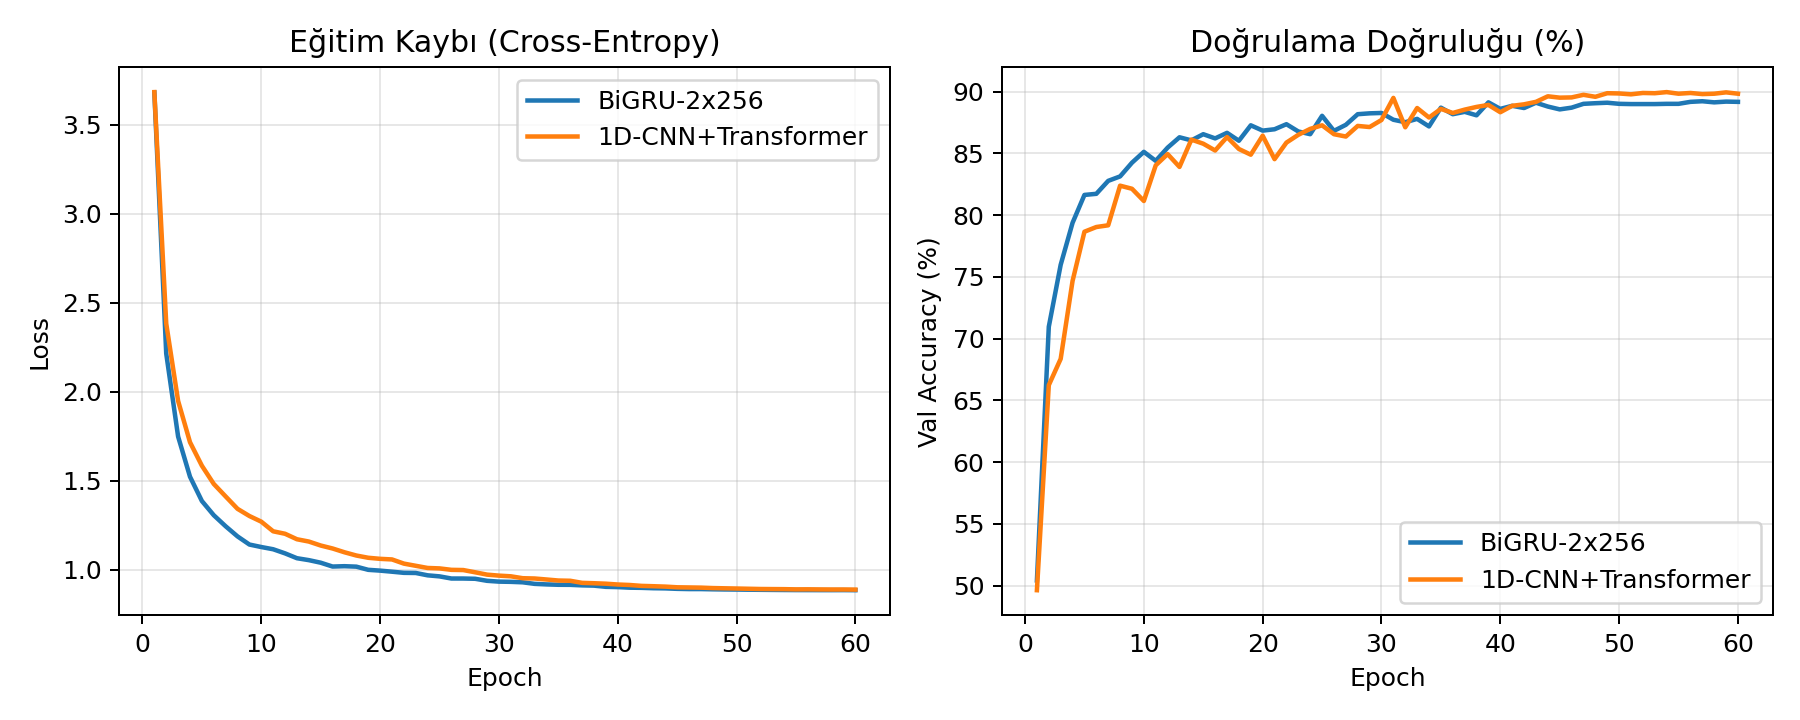
\includegraphics[width=\textwidth]{egitim_egrisi.png}
\end{column}
\end{columns}
\end{frame}

% 8
\begin{frame}{Ne elde ettik?}
\framesubtitle{Model: Mustafa Göktepe}
\centering
\begin{tabular}{@{}lrrrr@{}}
\toprule
\textbf{Model} & \textbf{Parametre} & \textbf{Doğrulama (\%)} & \textbf{Test (\%)} & \textbf{Macro F1 (\%)} \\
\midrule
BiGRU-2x256 & 2.114.018 & 89,23 & 88,24 & 88,09 \\
1B-CNN + Transformer & 1.473.634 & \textbf{89,97} & \textbf{88,83} & \textbf{88,61} \\
\bottomrule
\end{tabular}

\vspace{4mm}
\begin{tabular}{@{}lrr@{}}
\toprule
\textbf{Üç tohum (0, 1, 2)} & \textbf{Test ort.\ $\pm$ ss (\%)} & \textbf{Doğrulama ort.\ (\%)} \\
\midrule
BiGRU-2x256 & 87,98 $\pm$ 0,23 & 89,38 \\
1B-CNN + Transformer & \textbf{89,42 $\pm$ 0,52} & \textbf{90,37} \\
\bottomrule
\end{tabular}

\vspace{4mm}
\begin{itemize}
\item Tez önerisindeki yüzde 85 hedefini iki modelde de geçtik.
\item Küçük model üç tohumun üçünde de önde çıktı.
\end{itemize}
\end{frame}

% 9
\begin{frame}{Model nerede yanılıyor?}
\framesubtitle{Model: Mustafa Göktepe}
\begin{columns}[c]
\begin{column}{0.42\textwidth}
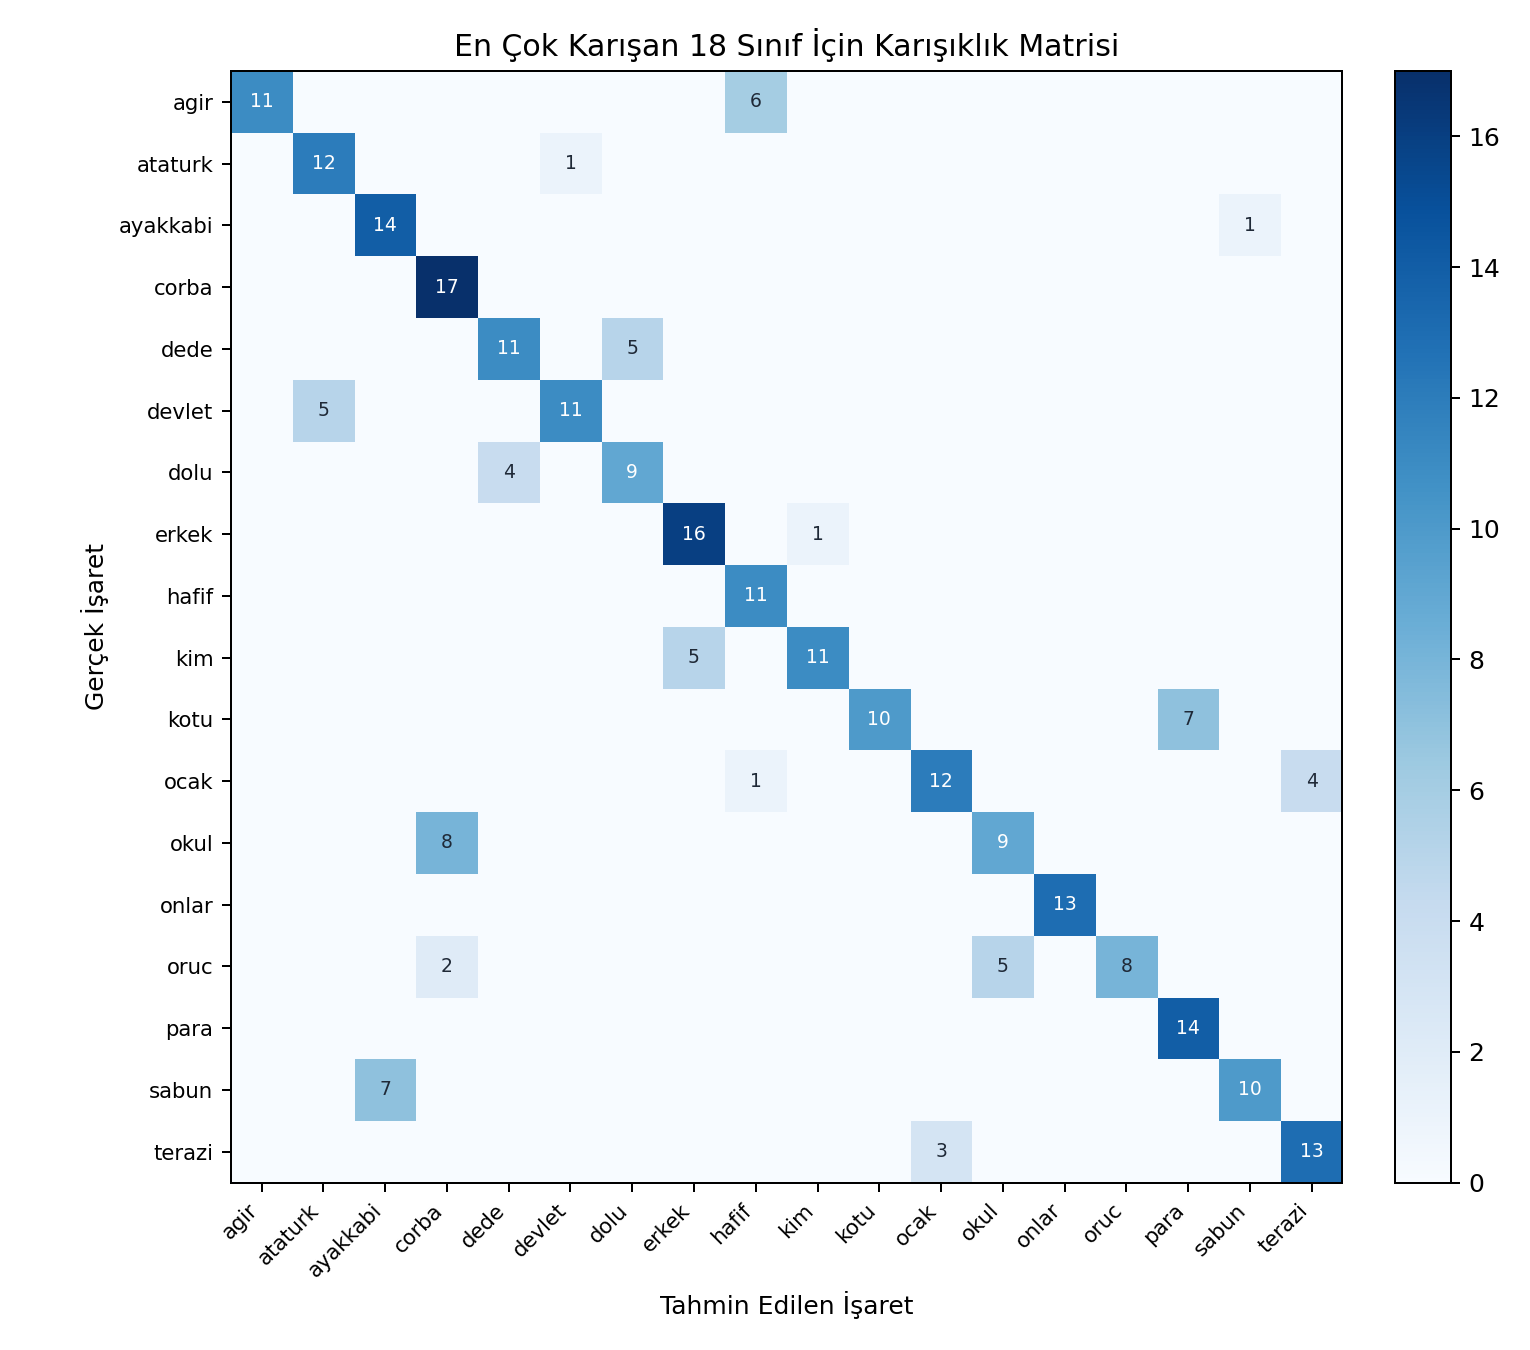
\includegraphics[width=\textwidth]{karisiklik_matrisi.png}
\end{column}
\begin{column}{0.56\textwidth}
\small
\begin{tabular}{@{}llr@{}}
\toprule
\textbf{Gerçek} & \textbf{Tahmin} & \textbf{Hata} \\
\midrule
okul & çorba & 8 / 17 \\
kötü & para & 7 / 17 \\
sabun & ayakkabı & 7 / 17 \\
ağır & hafif & 6 / 17 \\
\bottomrule
\end{tabular}

\vspace{4mm}
\begin{itemize}
\item Test kümesindeki 3.741 örnek için karışıklık matrisi çıkardık.
\item Hatalar rastgele değil: el formu ve konumu aynı olan işaretler karışıyor.
\item Güven eşiğini 0,6 seçtik: örneklerin yüzde 75'i kabul ediliyor, bunlarda doğruluk yüzde 96,8.
\end{itemize}
\end{column}
\end{columns}
\end{frame}

% 10
\begin{frame}{Modeli telefona nasıl taşıdık?}
\centering
\footnotesize
\setlength{\fboxsep}{4pt}
\fbox{PyTorch ağırlıkları} $\rightarrow$
\fbox{NumPy} $\rightarrow$
\fbox{Keras} $\rightarrow$
\fbox{LiteRT fp32} $\rightarrow$
\fbox{LiteRT int8}

\vspace{7mm}
\normalsize
\begin{itemize}
\item Dosya boyutu 9,43 MB'tan 3,19 MB'a indi; hedefimiz 10 MB'ın altıydı.
\item int8 sürümün test doğruluğu yüzde 88,0; kayıp yok.
\item Aynı 200 test örneğini hem Python'da hem telefonda çalıştırdık: tahminlerin yüzde 99,5'i aynı.
\end{itemize}
\end{frame}

% 11
\begin{frame}{Mobil uygulamayı nasıl kurduk?}
\framesubtitle{Mobil: Ahmet Çelik}
\begin{columns}[T]
\begin{column}{0.48\textwidth}
\textbf{Yapı}
\begin{itemize}
\item Kamera, MediaPipe ve LiteRT Kotlin tarafında (CameraX)
\item Ekranlar ve durum yönetimi Flutter'da
\item İki taraf olay kanallarıyla (event channel) konuşuyor
\item Model dosyası uygulamanın içinde, çevrimdışı çalışıyor
\end{itemize}
\end{column}
\begin{column}{0.48\textwidth}
\textbf{Ölçümler}
\begin{itemize}
\item Model çıkarımı ortalama 48 ms (Redmi Note 10 Pro)
\item Uçtan uca hız yaklaşık 9 FPS; hedef 15 FPS
\item Darboğaz model değil, kare başına çalışan iki MediaPipe modeli
\end{itemize}
\end{column}
\end{columns}
\end{frame}

% 12
\begin{frame}{Henüz çözemediklerimiz}
\begin{itemize}
\item \textbf{Canlı kamerada güven düşük.} Kayıtlı test verisinde yüzde 88--89 alırken canlı denemede tahmin güveni yüzde 3--20 aralığına düşüyor.
\item Neden henüz ayrışmadı: MediaPipe'ın canlı görüntüdeki nokta kalitesi, ön işleme farkı ya da segmentleme kuralları olabilir.
\item Planımız: aynı videoyu hem Python'da hem telefonda çıkarıp noktaları tek tek karşılaştırmak.
\end{itemize}

\vspace{3mm}
\begin{itemize}
\item \textbf{Hız hedefin altında.} 9 FPS'teyiz, hedef 15 FPS.
\end{itemize}
\end{frame}

% 13
\begin{frame}{Takvim ve sıradaki işler}
\centering
\small
\begin{tabular}{@{}lll@{}}
\toprule
\textbf{Kilometre taşı} & \textbf{Tarih} & \textbf{Durum} \\
\midrule
M0: depo, erişim, veri doğrulama & 29 Ekim & Tamamlandı \\
M1: nokta çıkarımı, iki modelin eğitimi, LiteRT & 7 Kasım & Tamamlandı \\
M2: ara rapor, karşılaştırma ve hata analizi & 20 Kasım & Devam ediyor \\
M3: üç tohum analizi, nihai model & 4 Aralık & Devam ediyor \\
M4: üç ekranlı uygulama, uçak modu testleri & 11 Aralık & Planlandı \\
M5: gönüllü testleri, performans ölçümleri & 18 Aralık & Planlandı \\
M6: tez teslimi & 1 Ocak & Planlandı \\
\bottomrule
\end{tabular}

\vspace{4mm}
\normalsize
\begin{itemize}
\item 1B-CNN + Transformer'ı da LiteRT int8'e aktarıp telefonda BiGRU ile karşılaştıracağız.
\item En az 30 işaret ve farklı kullanıcılarla gönüllü test protokolü hazırlayacağız.
\end{itemize}
\end{frame}

\end{document}
